\documentclass[tikz,border=8pt]{standalone}
% Shared look for every TikZ diagram. Load with % Shared look for every TikZ diagram. Load with % Shared look for every TikZ diagram. Load with \input{../../tools/tikz-style.tex}
\usepackage[T1]{fontenc}
\usepackage{lmodern}
\renewcommand{\sfdefault}{lmr}  % diagrams use the same serif as the text
\usetikzlibrary{arrows.meta, positioning, shapes.geometric, calc, fit, backgrounds}
\definecolor{cblue}{HTML}{4C78A8}
\definecolor{corange}{HTML}{F58518}
\definecolor{cgreen}{HTML}{54A24B}
\definecolor{cred}{HTML}{E45756}
\definecolor{cpurple}{HTML}{B279A2}
\definecolor{cgrey}{HTML}{6B6B6B}
\tikzset{
  every picture/.style={font=\sffamily, line width=1.2pt},
  box/.style={draw=#1, fill=#1!12, rounded corners=4pt, align=center, inner sep=7pt, minimum height=1.1cm},
  box/.default=cgrey,
  arrow/.style={-{Stealth[length=3mm]}, draw=cgrey, line width=1.4pt},
  title/.style={font=\sffamily\bfseries\Large},
  note/.style={font=\sffamily\small, text=cgrey, align=center},
}
\AtBeginDocument{\hyphenpenalty=10000 \exhyphenpenalty=10000}

\usepackage[T1]{fontenc}
\usepackage{lmodern}
\renewcommand{\sfdefault}{lmr}  % diagrams use the same serif as the text
\usetikzlibrary{arrows.meta, positioning, shapes.geometric, calc, fit, backgrounds}
\definecolor{cblue}{HTML}{4C78A8}
\definecolor{corange}{HTML}{F58518}
\definecolor{cgreen}{HTML}{54A24B}
\definecolor{cred}{HTML}{E45756}
\definecolor{cpurple}{HTML}{B279A2}
\definecolor{cgrey}{HTML}{6B6B6B}
\tikzset{
  every picture/.style={font=\sffamily, line width=1.2pt},
  box/.style={draw=#1, fill=#1!12, rounded corners=4pt, align=center, inner sep=7pt, minimum height=1.1cm},
  box/.default=cgrey,
  arrow/.style={-{Stealth[length=3mm]}, draw=cgrey, line width=1.4pt},
  title/.style={font=\sffamily\bfseries\Large},
  note/.style={font=\sffamily\small, text=cgrey, align=center},
}
\AtBeginDocument{\hyphenpenalty=10000 \exhyphenpenalty=10000}

\usepackage[T1]{fontenc}
\usepackage{lmodern}
\renewcommand{\sfdefault}{lmr}  % diagrams use the same serif as the text
\usetikzlibrary{arrows.meta, positioning, shapes.geometric, calc, fit, backgrounds}
\definecolor{cblue}{HTML}{4C78A8}
\definecolor{corange}{HTML}{F58518}
\definecolor{cgreen}{HTML}{54A24B}
\definecolor{cred}{HTML}{E45756}
\definecolor{cpurple}{HTML}{B279A2}
\definecolor{cgrey}{HTML}{6B6B6B}
\tikzset{
  every picture/.style={font=\sffamily, line width=1.2pt},
  box/.style={draw=#1, fill=#1!12, rounded corners=4pt, align=center, inner sep=7pt, minimum height=1.1cm},
  box/.default=cgrey,
  arrow/.style={-{Stealth[length=3mm]}, draw=cgrey, line width=1.4pt},
  title/.style={font=\sffamily\bfseries\Large},
  note/.style={font=\sffamily\small, text=cgrey, align=center},
}
\AtBeginDocument{\hyphenpenalty=10000 \exhyphenpenalty=10000}

\begin{document}
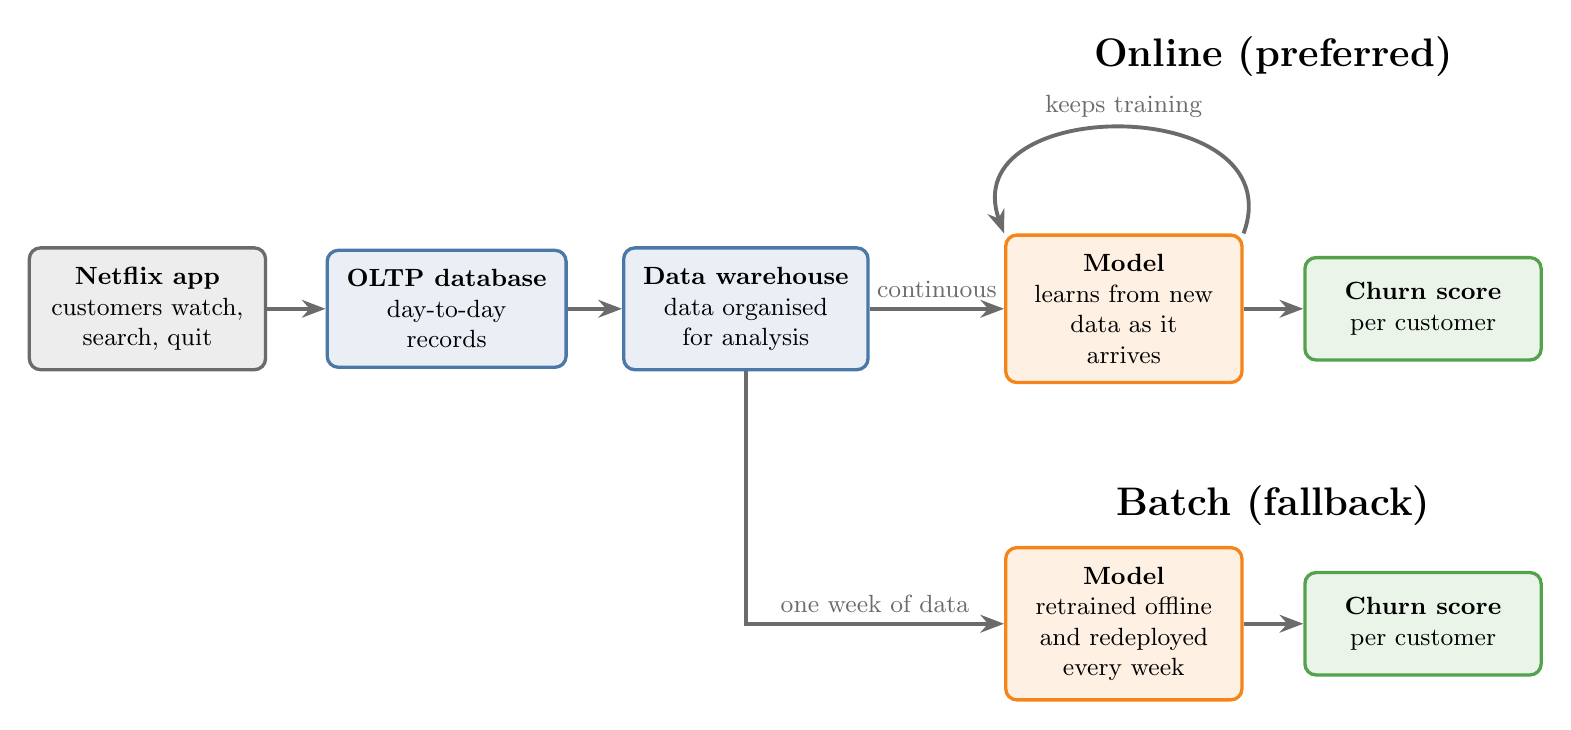
\begin{tikzpicture}
  \tikzset{b/.style={box=#1, minimum width=3.0cm, minimum height=1.3cm, font=\small}}
  % shared data flow
  \node[b=cgrey] (app) at (0,0) {\textbf{Netflix app}\\customers watch,\\search, quit};
  \node[b=cblue] (oltp) at (3.8,0) {\textbf{OLTP database}\\day-to-day\\records};
  \node[b=cblue] (dw) at (7.6,0) {\textbf{Data warehouse}\\data organised\\for analysis};
  \draw[arrow] (app) -- (oltp);
  \draw[arrow] (oltp) -- (dw);
  % online
  \node[title] at (14.3,3.2) {Online (preferred)};
  \node[b=corange] (mo) at (12.4,0) {\textbf{Model}\\learns from new\\data as it\\arrives};
  \node[b=cgreen] (so) at (16.2,0) {\textbf{Churn score}\\per customer};
  \draw[arrow] (dw) -- node[note, above] {continuous} (mo);
  \draw[arrow] (mo) -- (so);
  \draw[arrow] (mo.north east) to[out=70, in=110, looseness=1.6] node[note, above] {keeps training} (mo.north west);
  % batch
  \node[title] at (14.3,-2.5) {Batch (fallback)};
  \node[b=corange] (mb) at (12.4,-4.0) {\textbf{Model}\\retrained offline\\and redeployed\\every week};
  \node[b=cgreen] (sb) at (16.2,-4.0) {\textbf{Churn score}\\per customer};
  \draw[arrow] (dw) |- node[note, pos=0.75, above] {one week of data} (mb);
  \draw[arrow] (mb) -- (sb);
\end{tikzpicture}
\end{document}
